% A LaTeX template for MSc Thesis submissions to 
% Politecnico di Milano (PoliMi) - School of Industrial and Information Engineering
%
% Copyright 2021 Politecnico di Milano, Italy. NC-BY

\documentclass{Configuration_Files/PoliMi3i_thesis}

%------------------------------------------------------------------------------
%	REQUIRED PACKAGES AND  CONFIGURATIONS
%------------------------------------------------------------------------------

% CONFIGURATIONS
\usepackage{parskip} % For paragraph layout
\usepackage{setspace} % For using single or double spacing
\usepackage{emptypage} % To insert empty pages
\usepackage{minted}
\usepackage{multicol} % To write in multiple columns (executive summary)
\setlength\columnsep{15pt} % Column separation in executive summary
\setlength\parindent{0pt} % Indentation
\raggedbottom  


% PACKAGES FOR TITLES
\usepackage{titlesec}
% \titlespacing{\section}{left spacing}{before spacing}{after spacing}
\titlespacing{\section}{0pt}{3.3ex}{2ex}
\titlespacing{\subsection}{0pt}{3.3ex}{1.65ex}
\titlespacing{\subsubsection}{0pt}{3.3ex}{1ex}
\usepackage{color}

% PACKAGES FOR LANGUAGE AND FONT
\usepackage[english]{babel} % The document is in English  
\usepackage[utf8]{inputenc} % UTF8 encoding
\usepackage[T1]{fontenc} % Font encoding
\usepackage[11pt]{moresize} % Big fonts

% PACKAGES FOR IMAGES
\usepackage{graphicx}
\usepackage{transparent} % Enables transparent images
\usepackage{eso-pic} % For the background picture on the title page
\usepackage{subfig} % Numbered and caption subfigures using \subfloat.
\usepackage{tikz} % A package for high-quality hand-made figures.
\usetikzlibrary{}
\graphicspath{{./Images/}} % Directory of the images
\usepackage{caption} % Coloured captions
\usepackage{xcolor} % Coloured captions
\usepackage{amsthm,thmtools,xcolor} % Coloured "Theorem"
\usepackage{float}
\usepackage{hyperref}

% STANDARD MATH PACKAGES
\usepackage{amsmath}
\usepackage{amsthm}
\usepackage{amssymb}
\usepackage{amsfonts}
\usepackage{bm}
\usepackage[overload]{empheq} % For braced-style systems of equations.
\usepackage{fix-cm} % To override original LaTeX restrictions on sizes

% PACKAGES FOR TABLES
\usepackage{tabularx}
\usepackage{longtable} % Tables that can span several pages
\usepackage{colortbl}

% PACKAGES FOR ALGORITHMS (PSEUDO-CODE)
\usepackage{algorithm}
\usepackage{algorithmic}

% PACKAGES FOR REFERENCES & BIBLIOGRAPHY
\usepackage[colorlinks=true,linkcolor=black,anchorcolor=black,citecolor=black,filecolor=black,menucolor=black,runcolor=black,urlcolor=black]{hyperref} % Adds clickable links at references
\usepackage{cleveref}
\usepackage[square, numbers, sort&compress]{natbib} % Square brackets, citing references with numbers, citations sorted by appearance in the text and compressed
\bibliographystyle{abbrvnat} % You may use a different style adapted to your field

% OTHER PACKAGES
\usepackage{pdfpages} % To include a pdf file
\usepackage{afterpage}
\usepackage{lipsum} % DUMMY PACKAGE
\usepackage{fancyhdr} % For the headers
\fancyhf{}

% Input of configuration file. Do not change config.tex file unless you really know what you are doing. 
% Define blue color typical of polimi
\definecolor{bluepoli}{cmyk}{0.4,0.1,0,0.4}

% Custom theorem environments
\declaretheoremstyle[
  headfont=\color{bluepoli}\normalfont\bfseries,
  bodyfont=\color{black}\normalfont\itshape,
]{colored}

% Set-up caption colors
\captionsetup[figure]{labelfont={color=bluepoli}} % Set colour of the captions
\captionsetup[table]{labelfont={color=bluepoli}} % Set colour of the captions
\captionsetup[algorithm]{labelfont={color=bluepoli}} % Set colour of the captions

\theoremstyle{colored}
\newtheorem{theorem}{Theorem}[chapter]
\newtheorem{proposition}{Proposition}[chapter]

% Enhances the features of the standard "table" and "tabular" environments.
\newcommand\T{\rule{0pt}{2.6ex}}
\newcommand\B{\rule[-1.2ex]{0pt}{0pt}}

% Pseudo-code algorithm descriptions.
\newcounter{algsubstate}
\renewcommand{\thealgsubstate}{\alph{algsubstate}}
\newenvironment{algsubstates}
  {\setcounter{algsubstate}{0}%
   \renewcommand{\STATE}{%
     \stepcounter{algsubstate}%
     \Statex {\small\thealgsubstate:}\space}}
  {}

% New font size
\newcommand\numfontsize{\@setfontsize\Huge{200}{60}}

% Title format: chapter
\titleformat{\chapter}[hang]{
\fontsize{50}{20}\selectfont\bfseries\filright}{\textcolor{bluepoli} \thechapter\hsp\hspace{2mm}\textcolor{bluepoli}{|   }\hsp}{0pt}{\huge\bfseries \textcolor{bluepoli}
}

% Title format: section
\titleformat{\section}
{\color{bluepoli}\normalfont\Large\bfseries}
{\color{bluepoli}\thesection.}{1em}{}

% Title format: subsection
\titleformat{\subsection}
{\color{bluepoli}\normalfont\large\bfseries}
{\color{bluepoli}\thesubsection.}{1em}{}

% Title format: subsubsection
\titleformat{\subsubsection}
{\color{bluepoli}\normalfont\large\bfseries}
{\color{bluepoli}\thesubsubsection.}{1em}{}

% Shortening for setting no horizontal-spacing
\newcommand{\hsp}{\hspace{0pt}}

\makeatletter
% Renewcommand: cleardoublepage including the background pic
\renewcommand*\cleardoublepage{%
  \clearpage\if@twoside\ifodd\c@page\else
  \null
  \AddToShipoutPicture*{\BackgroundPic}
  \thispagestyle{empty}%
  \newpage
  \if@twocolumn\hbox{}\newpage\fi\fi\fi}
\makeatother

%For correctly numbering algorithms
\numberwithin{algorithm}{chapter}

%----------------------------------------------------------------------------
%	NEW COMMANDS DEFINED
%----------------------------------------------------------------------------

% EXAMPLES OF NEW COMMANDS
\newcommand{\bea}{\begin{eqnarray}} % Shortcut for equation arrays
\newcommand{\eea}{\end{eqnarray}}
\newcommand{\e}[1]{\times 10^{#1}}  % Powers of 10 notation

%----------------------------------------------------------------------------
%	ADD YOUR PACKAGES (be careful of package interaction)
%----------------------------------------------------------------------------

%----------------------------------------------------------------------------
%	ADD YOUR DEFINITIONS AND COMMANDS (be careful of existing commands)
%----------------------------------------------------------------------------

%----------------------------------------------------------------------------
%	BEGIN OF YOUR DOCUMENT
%----------------------------------------------------------------------------

\begin{document}

\fancypagestyle{plain}{%
\fancyhf{} % Clear all header and footer fields
\fancyhead[RO,RE]{\thepage} %RO=right odd, RE=right even
\renewcommand{\headrulewidth}{0pt}
\renewcommand{\footrulewidth}{0pt}}

%----------------------------------------------------------------------------
%	TITLE PAGE
%----------------------------------------------------------------------------

\pagestyle{empty} % No page numbers
\frontmatter % Use roman page numbering style (i, ii, iii, iv...) for the preamble pages

\puttitle{
	title=Systems and Methods for Big and Unstructured Data Project,
	name1=Angelo Prete,
	name2=Antonio Riverso, 
	name3=Andrea Sanvito,
	academicyear=2024-2025,
	groupnumber=32
} % These info will be put into your Title page 

%----------------------------------------------------------------------------
%	PREAMBLE PAGES: ABSTRACT (inglese e italiano), EXECUTIVE SUMMARY
%----------------------------------------------------------------------------
\startpreamble
\setcounter{page}{1} % Set page counter to 1

%----------------------------------------------------------------------------
%	LIST OF CONTENTS/FIGURES/TABLES/SYMBOLS
%----------------------------------------------------------------------------

% TABLE OF CONTENTS
\thispagestyle{empty}
\tableofcontents % Table of contents 
\thispagestyle{empty}
\cleardoublepage

%-------------------------------------------------------------------------
%	THESIS MAIN TEXT
%-------------------------------------------------------------------------
% In the main text of your thesis you can write the chapters in two different ways:
%
%(1) As presented in this template you can write:
%    \chapter{Title of the chapter}
%    *body of the chapter*
%
%(2) You can write your chapter in a separated .tex file and then include it in the main file with the following command:
%    \chapter{Title of the chapter}
%    \input{chapter_file.tex}
%
% Especially for long thesis, we recommend you the second option.

\addtocontents{toc}{\vspace{2em}} % Add a gap in the Contents, for aesthetics
\mainmatter % Begin numeric (1,2,3...) page numbering

\chapter{Introduction}

For the project, we decided to analyze two datasets, the Formula 1 dataset and the Letterboxd dataset. Both of them can be found at Kaggle.

\section{Letterbox Database}

Our first analysis is on the \href{https://www.kaggle.com/datasets/gsimonx37/letterboxd}{Letterboxd Movies Dataset}, that is a comprehensive collection of movie-related data derived from the \href{https://letterboxd.com/}{Letterboxd} website. It contains information about movies, such as titles, release dates, genres, average ratings, directors, actors, studios, and production details.

The raw dataset was cleaned and processed using a Python script. This script replaced unsupported characters in the CSV files to ensure compatibility with the database. After cleaning, we imported the dataset into a Neo4j database, creating nodes for movies, actors, genres, and studios, and establishing relationships like actors starring in movies and genres linked to films.

We decided to use Neo4j since it makes the process of querying connected data like movies, actors and directors simple. The queries rely heavily on relationships—such as finding actor-director pairings or tracking genre trends over time—and Neo4j is designed to navigate these links efficiently. Since it is schema-free handling data like ours with a lot of missing values becomes easier. Additionally, importing and linking data from CSV files is very straightforward.

\section{Formula 1 Database}
Our second analysis focuses on a \href{https://www.kaggle.com/datasets/rohanrao/formula-1-world-championship-1950-2020}{dataset of Formula 1} records. In particular, it includes the results of all Formula 1 sessions (races, qualifying rounds, sprint races, etc.) over the years, together with supplementary data such as pit stop durations and race lap times.

As with the previous case, the raw dataset was cleaned and processed using Python. However, this time it required additional effort. For example we chose to import it after removing non-essential fields, such as links to Wikipedia pages related to different entities.

We decided to exploit MongoDB's functionalities to query the dataset, as the structure of races and championships aligns naturally with the document-oriented model of Documental databases. Additionally, the schema-less nature of MongoDB allowed us to eliminate all null values.

\chapter{Data Wrangling}
\section{Letterbox dataset data wrangling}
In order to ensure clean and consistent CSV data for import into Neo4j, we performed 
a small data wrangling step in Python by using the following function. This step replaced any irregular escaped quotes 
(e.g. \texttt{\textbackslash \"}) in our raw CSV files with standard quotes, preventing 
errors during loading.

\subsection*{Python Script for Cleaning CSV Files}

\inputminted{python}{letterboxd/letterboxdDataCleaning.py}

\section{Formula 1 dataset data wrangling}
As of the Formula 1 dataset, it was processed through another Python script.

The CSV files were loaded with the \textit{csv} Python module, processed through dictionaries, and dumped into a JSON file using the \textit{json} Python module.

Additionally, null values were addressed through the same Python script simply by not adding the related field.

As the script is fairly extensive (around 400 lines of code), we only reported examples of helper functions, \textit{time\_to\_milliseconds}, load functions, \textit{load\_qualifyings}, and the unifying "wrapper" function, \textit{build\_championships}.

\subsection*{Python Script for Processing CSV Files}

\inputminted{python}{formula1/formula1QualiWrangling.py}

\chapter{Dataset}

\section{Letterbox dataset}

As stated in the dataset page on Kaggle, the dataset is provided through csv files with the following structure:

\begin{itemize}
    \item \textbf{movies.csv} - Basic information about films:
    \begin{itemize}
        \item \textit{id} - Movie identifier (primary key);
        \item \textit{name} - The name of the film;
        \item \textit{date} - Year of release of the film;
        \item \textit{tagline} - The slogan of the film;
        \item \textit{description} - Description of the film;
        \item \textit{minute} - Movie duration (in minutes);
        \item \textit{rating} - Average rating of the film.
    \end{itemize}
    \item \textbf{actors.csv} - Actors who took part in the filming of films:
    \begin{itemize}
        \item \textit{id} - Movie identifier (foreign key);
        \item \textit{name} - Name;
        \item \textit{role} - Role.
    \end{itemize}
    \item \textbf{crew.csv} - Film crew:
    \begin{itemize}
        \item \textit{id} - Movie identifier (foreign key);
        \item \textit{role} - Role in the film crew (director, screenwriter, etc.);
        \item \textit{name} - Name.
    \end{itemize}
    \item \textbf{languages.csv} - In what languages the films were shot:
    \begin{itemize}
        \item \textit{id} - Movie identifier (foreign key);
        \item \textit{type} - Type (primary, conversational, etc.);
        \item \textit{language} - Film language.
    \end{itemize}
    \item \textbf{studios.csv} - Film studios:
    \begin{itemize}
        \item \textit{id} - Movie identifier (foreign key);
        \item \textit{studio} - Film studio.
    \end{itemize}
    \item \textbf{countries.csv} - Countries:
    \begin{itemize}
        \item \textit{id} - Movie identifier (foreign key);
        \item \textit{country} - Country.
    \end{itemize}
    \item \textbf{genres.csv} - Film genres:
    \begin{itemize}
        \item \textit{id} - Movie identifier (foreign key);
        \item \textit{genre} - Film genre.
    \end{itemize}
    \item \textbf{themes.csv} - Themes in films:
    \begin{itemize}
        \item \textit{id} - Movie identifier (foreign key);
        \item \textit{theme} - The theme of the film.
    \end{itemize}
    \item \textbf{releases.csv} - Movie releases:
    \begin{itemize}
        \item \textit{id} - Movie identifier (foreign key);
        \item \textit{country} - Release country;
        \item \textit{date} - Release date of the film;
        \item \textit{type} - Release type (theatrical, television, etc.) of the film;
        \item \textit{rating} - Age rating of the film.
    \end{itemize}
    \item \textbf{posters.csv} - Movie posters:
    \begin{itemize}
        \item \textit{id} - Movie identifier (foreign key);
        \item \textit{country} - URL address.
    \end{itemize}
\end{itemize}

Since we don't need the posters for our analysis, we didn't import it in our Neo4j instance.

We first created the following indexes to speed-up both imports and queries:

\inputminted[frame=single,framesep=10pt,breaklines]{cypher}{letterboxd/import/index.cypher}

CSV files were imported using the following commands (through peridic commits, given their sizes):

first of all we imported the movies

\inputminted[frame=single,framesep=10pt,breaklines]{cypher}{letterboxd/import/movies.cypher}

then, all the other tables (linked through the foreign key movie id, which is present in each row)

\inputminted[frame=single,framesep=10pt,breaklines]{cypher}{letterboxd/import/actors.cypher}
\inputminted[frame=single,framesep=10pt,breaklines]{cypher}{letterboxd/import/crew.cypher}
\inputminted[frame=single,framesep=10pt,breaklines]{cypher}{letterboxd/import/languages.cypher}
\inputminted[frame=single,framesep=10pt,breaklines]{cypher}{letterboxd/import/studio.cypher}
\inputminted[frame=single,framesep=10pt,breaklines]{cypher}{letterboxd/import/country.cypher}
\inputminted[frame=single,framesep=10pt,breaklines]{cypher}{letterboxd/import/genre.cypher}
\inputminted[frame=single,framesep=10pt,breaklines]{cypher}{letterboxd/import/theme.cypher}

for releases, we didn't create new nodes; instead, we used the existing Country nodes and added "RElEASED\_IN" relationships between movies and countries

\inputminted[frame=single,framesep=10pt,breaklines]{cypher}{letterboxd/import/release.cypher}

An example of the produced structure can be seen in figure \ref{fig:graph_example}, where we show some nodes (one of each type present in the database) related to the movie "The Wolf of Wall Street".
\newpage
\begin{figure}[!h]
    \centering
    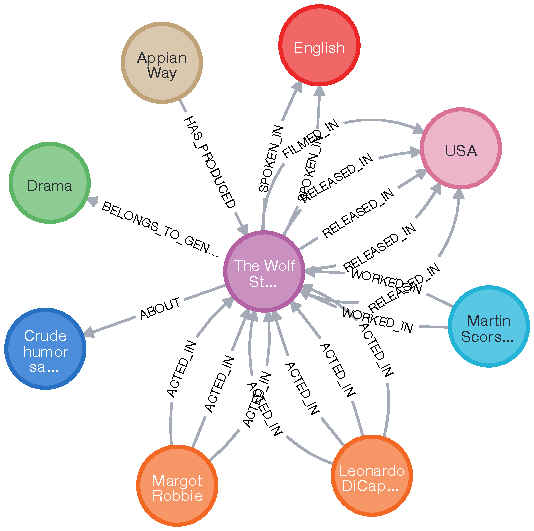
\includegraphics[width=0.6\linewidth]{latex/letterboxd/graph_example.pdf}
    \caption{Truncated graph of "The Wolf of Wall Street" movie}
    \label{fig:graph_example}
\end{figure}

\newpage
\section{Formula 1 dataset}
As already mentioned, the dataset was taken from Kaggle. It can be found as a list of CSV files with the following structure:

\begin{itemize}
    \item \textbf{circuits.csv} - Circuits in which at least one race has taken place:
    \begin{itemize}
        \item \textit{circuitId} - Circuit identifier (primary key);
        \item \textit{circuitRef} - Reference string for the circuit;
        \item \textit{name} - Name of the circuit;
        \item \textit{location} - City in which the circuit is located;
        \item \textit{country} - Country in which the circuit is located;
        \item \textit{lat} - Latitude coordinate;
        \item \textit{lng} - Longitude coordinate;
        \item \textit{alt} - Altitude coordinate;
        \item \textit{url} - Link to the Wikipedia page of the circuit;
    \end{itemize}

    \item \textbf{constructor\_results.csv} - Results and points for constructors after each race:
    \begin{itemize}
        \item \textit{constructorResultsId} - Result identifier (primary key);
        \item \textit{raceId} - Race identifier (foreign key);
        \item \textit{constructorId} - Constructor identifier (foreign key);
        \item \textit{points} - Count of points obtained by the race;
        \item \textit{status} - Status of the constructor after the race;
    \end{itemize}

    \item \textbf{constructor\_standings.csv} - Constructors standings after each race:
    \begin{itemize}
        \item \textit{constructorStandingsId} - Standings entry identifier (primary key);
        \item \textit{raceId} - Race identifier (foreign key);
        \item \textit{constructorId} - Constructor identifier (foreign key);
        \item \textit{points} - Count of points after the race;
        \item \textit{position} - Position in the standings;
        \item \textit{positionText} - Text version of the previous field;
        \item \textit{wins} - Count of wins so far;
    \end{itemize}

    \item \textbf{constructors.csv} - Constructors general information:
    \begin{itemize}
        \item \textit{constructorId} - Constructor identifier (primary key);
        \item \textit{constructorRef} - Refernce string for the constructor;
        \item \textit{name} - Name of the constructor;
        \item \textit{nationality} - Name of the constructor;
        \item \textit{url} - Link to the Wikipedia page of the constructor;
    \end{itemize}

    \item \textbf{driver\_standings.csv} - Driver standings after each race:
    \begin{itemize}
        \item \textit{driverStandingsId} - Standings entry identifier (primary key);
        \item \textit{raceId} - Race identifier (foreign key);
        \item \textit{driverId} - Driver identifier (foreign key);
        \item \textit{points} - Count of points after the race;
        \item \textit{position} - Position in the standings;
        \item \textit{positionText} - Text version of the previous field;
        \item \textit{wins} - Count of wins so far;
    \end{itemize}

    \item \textbf{drivers.csv} - Drivers general information:
    \begin{itemize}
        \item \textit{driverId} - Driver identifier (primary key);
        \item \textit{driverRef} - Reference string for the driver;
        \item \textit{number} - Number on the car of the driver;
        \item \textit{code} - Code used to display the driver during the races;
        \item \textit{forename} - Name of the driver;
        \item \textit{surname} - Surname of the driver;
        \item \textit{dob} - Date of birth of the driver;
        \item \textit{nationality} - Nationality of the driver;
        \item \textit{url} - Link to the Wikipedia page of the driver;
    \end{itemize}

    \item \textbf{lap\_times.csv} - Lap times registered at every session:
    \begin{itemize}
        \item \textit{raceId} - Race identifier (foreign key);
        \item \textit{driverId} - Driver identifier (foreign key);
        \item \textit{lap} - Lap of the race the time was registered in;
        \item \textit{position} - Position in which the driver registered the time;
        \item \textit{time} - Time of the lap (mm:ss.ms format);
        \item \textit{milliseconds} - Time of the lap (in milliseconds);
    \end{itemize}

    \item \textbf{pit\_stops.csv} - Information about pit stops taken in every race:
    \begin{itemize}
        \item \textit{raceId} - Race identifier (foreign key);
        \item \textit{driverId} - Driver identifier (foreign key);
        \item \textit{stop} - Counter of the stops;
        \item \textit{lap} - Lap of the race the pit stop was taken in;
        \item \textit{duration} - Duration of the pit stop (mm:ss.ms format);
        \item \textit{milliseconds} - Duration of the pit stop (in milliseconds);
    \end{itemize}

    \item \textbf{qualifying.csv} - Results of qualifying sessions:
    \begin{itemize}
        \item \textit{qualifyId} - Qualifying entry identifier (primary key);
        \item \textit{raceId} - Race identifier (foreign key);
        \item \textit{driverId} - Driver identifier (foreign key);
        \item \textit{constructorId} - Constructor identifier (foreign key);
        \item \textit{number} - Number on the car of the driver;
        \item \textit{position} - Position in which the driver qualified;
        \item \textit{q1} - Lap time registered in the first qualifying session;
        \item \textit{q2} - Lap time registered in the second qualifying session;
        \item \textit{q3} - Lap time registered in the third qualifying session;
    \end{itemize}

    \item \textbf{races.csv} - General information about race sessions:
    \begin{itemize}
        \item \textit{raceId} - Race identifier (primary key);
        \item \textit{year} - Year in which the race took place;
        \item \textit{round} - Number representing what round in the championship the race is;
        \item \textit{circuitId} - Circuit identifier (foreign key);
        \item \textit{name} - Name of the race;
        \item \textit{date} - Date in which the race takes place;
        \item \textit{time} - Time at which the race takes place;
        \item \textit{url} - Link to the Wikipedia page of the race;
        \item \textit{fp1\_date} - Date of the first practice session;
        \item \textit{fp1\_time} - Time of the first practice session;
        \item \textit{fp2\_date} - Date of the second practice session;
        \item \textit{fp2\_time} - Time of the second practice session;
        \item \textit{fp3\_date} - Date of the third practice session;
        \item \textit{fp3\_time} - Time of the third practice session;
        \item \textit{quali\_date} - Date of the qualifying session;
        \item \textit{quali\_time} - Time of the qualifying session;
        \item \textit{sprint\_date} - Date of the sprint session;
        \item \textit{sprint\_time} - Time of the sprint session;
    \end{itemize}

    \item \textbf{results.csv} - Results of the race sessions:
    \begin{itemize}
        \item \textit{resultId} - Identifier for the single entry (primary key);
        \item \textit{raceId} - Race identifier (foreign key);
        \item \textit{driverId} - Driver identifier (foreign key);
        \item \textit{constructorId} - Constructor identifier (foreign key);
        \item \textit{number} - Number on the car of the driver;
        \item \textit{grid} - Starting position for the driver;
        \item \textit{position} - Finishing position for the driver;
        \item \textit{positionText} - Text version of the previous field;
        \item \textit{positionOrder} - Position in the finishing order;
        \item \textit{points} - Points gained by the driver;
        \item \textit{laps} - Laps done by the driver;
        \item \textit{time} - Time it took the driver to finish the race (hh:mm::ss.ms format);
        \item \textit{milliseconds} - Time it took the driver to finish the race (in milliseconds);
        \item \textit{fastestLap} - Lap in which the driver recorded his best lap time;
        \item \textit{rank} - Rank of the fastest lap recorded;
        \item \textit{fastestLapTime} - Time of the fastest lap (mm:ss.ms format);
        \item \textit{fastestLapSpeed} - Average speed of the driver during the fastest lap;
        \item \textit{status} - Status of the driver at the end of the race;
    \end{itemize}

    \item \textbf{seasons.csv} - General information of the F1 seasons:
    \begin{itemize}
        \item \textit{year} - Year of the season (primary key);
        \item \textit{url} - Link to the Wikipedia page of the season;
    \end{itemize}

    \item \textbf{sprint\_results.csv} - Results of the sprints sessions:
    \begin{itemize}
        \item \textit{resultId} - Identifier for the single entry (primary key);
        \item \textit{raceId} - Race identifier (foreign key);
        \item \textit{driverId} - Driver identifier (foreign key);
        \item \textit{constructorId} - Constructor identifier (foreign key);
        \item \textit{number} - Number on the car of the driver;
        \item \textit{grid} - Starting position for the driver;
        \item \textit{position} - Finishing position for the driver;
        \item \textit{positionText} - Text version of the previous field;
        \item \textit{positionOrder} - Position in the finishing order;
        \item \textit{points} - Points gained by the driver;
        \item \textit{laps} - Laps done by the driver;
        \item \textit{time} - Time it took the driver to finish the sprint (hh:mm::ss.ms format);
        \item \textit{milliseconds} - Time it took the driver to finish the sprint (in milliseconds);
        \item \textit{fastestLap} - Lap in which the driver recorded his best lap time;
        \item \textit{fastestLapTime} - Time of the fastest lap (mm:ss.ms format);
        \item \textit{status} - Status of the driver at the end of the sprint;
    \end{itemize}

    \item \textbf{status.csv} - Possible driver statuses at the end of a session:
    \begin{itemize}
        \item \textit{statusId} - Status identifier (primary key);
        \item \textit{status} - Status of the driver;
    \end{itemize}
\end{itemize}

The entire \textbf{lap\_times} and \textbf{constructor\_results} files were excluded as they were not relevant to our queries. All data was processed to align more closely with the Document-oriented approach.

\subsection*{Importing data into MongoDB}
To store data into MongoDB Atlas, we created a database named \textbf{formula-1} and a collection named \textbf{championships}.

Excluding the functions for loading CSV files into Python (as outlined in Section 2.2), additional scripts were employed to convert the data to JSON format and import them into the database. The two principal functions are shown below.

\vspace{0.5cm}
\inputminted{python}{formula1/export.py}

\vspace{0.5cm}
\inputminted{python}{formula1/import.py}



\chapter{Queries}

\section{Letterbox dataset queries}

\subsection{Average rating, length and number of movies over the years}

With this query we calculated the average rating, duration, and number of movies released each year for films over 60 minutes, excluding those from 2024 (since the dataset is incomplete for the year). It helped us identify trends in movie quality and length over time, as plotted in the graphs below.

\inputminted[frame=single,framesep=10pt,breaklines]{cypher}{letterboxd/queries/query1.cypher}

The query returns the following (truncated) result:

\begin{table}[h!]
\centering
\begin{tabular}{|c|c|c|c|}
\hline
\textbf{year} & \textbf{avg\_rating} & \textbf{avg\_duration} & \textbf{n\_movies} \\ \hline
2023 & 3.18 & 121.77 & 15598 \\ \hline
2022 & 3.15 & 125.01 & 14869 \\ \hline
2021 & 3.17 & 122.92 & 13841 \\ \hline
2020 & 3.15 & 120.36 & 12372 \\ \hline
2019 & 3.16 & 114.06 & 14173 \\ \hline
2018 & 3.14 & 112.90 & 13473 \\ \hline
2017 & 3.14 & 111.82 & 12963 \\ \hline
\end{tabular}
\caption{Average Rating, Duration, and Number of Movies by Year}
\end{table}

\begin{figure}[!h]
  \centering
  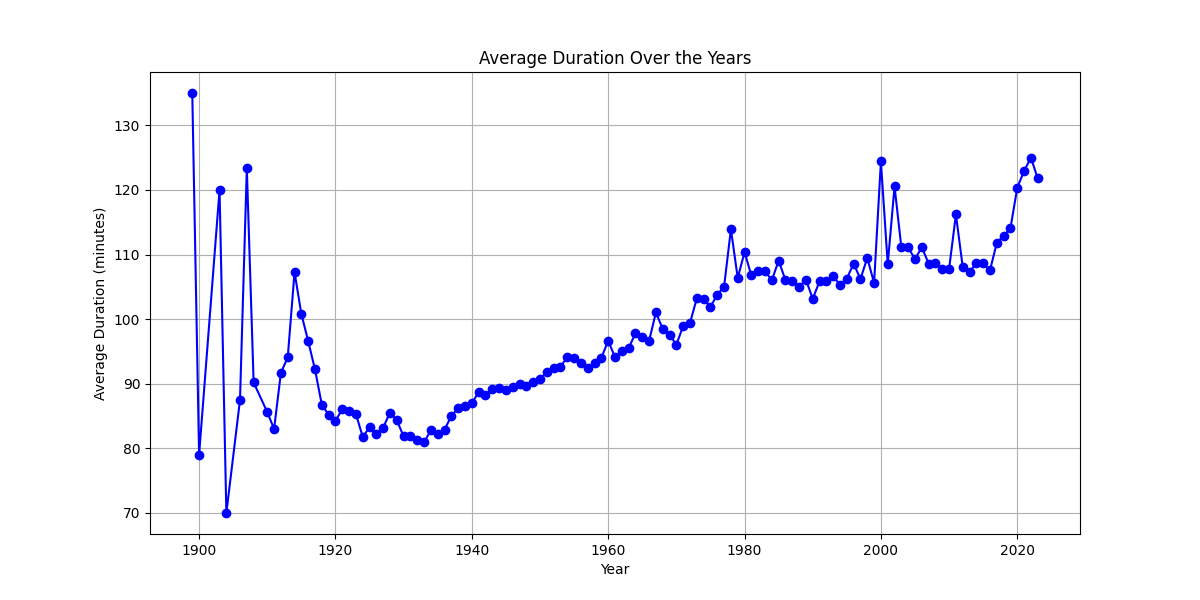
\includegraphics[width=\textwidth]{latex/letterboxd/visualization/average_duration_trend.png}
  \caption{Average movie duration trend.}
  \label{fig:duration_trend}
\end{figure}

\begin{figure}[!h]
  \centering
  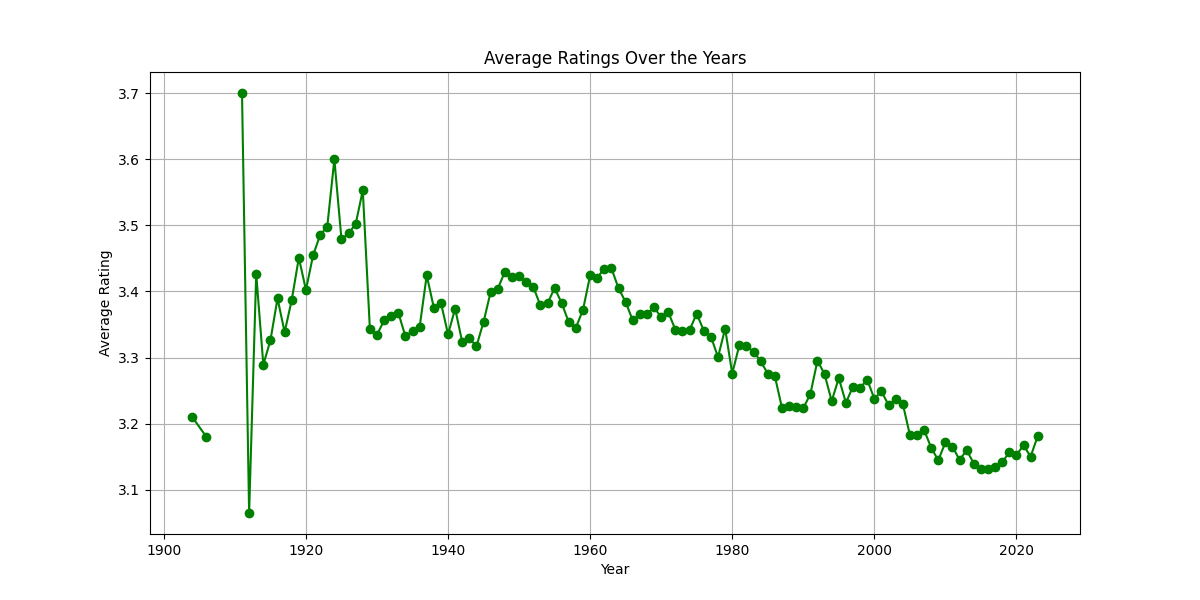
\includegraphics[width=\textwidth]{latex/letterboxd/visualization/average_ratings_trend.png}
  \caption{Average movie ratings trend.}
  \label{fig:ratings_trend}
\end{figure}
\clearpage
\begin{figure}[H]
  \centering
  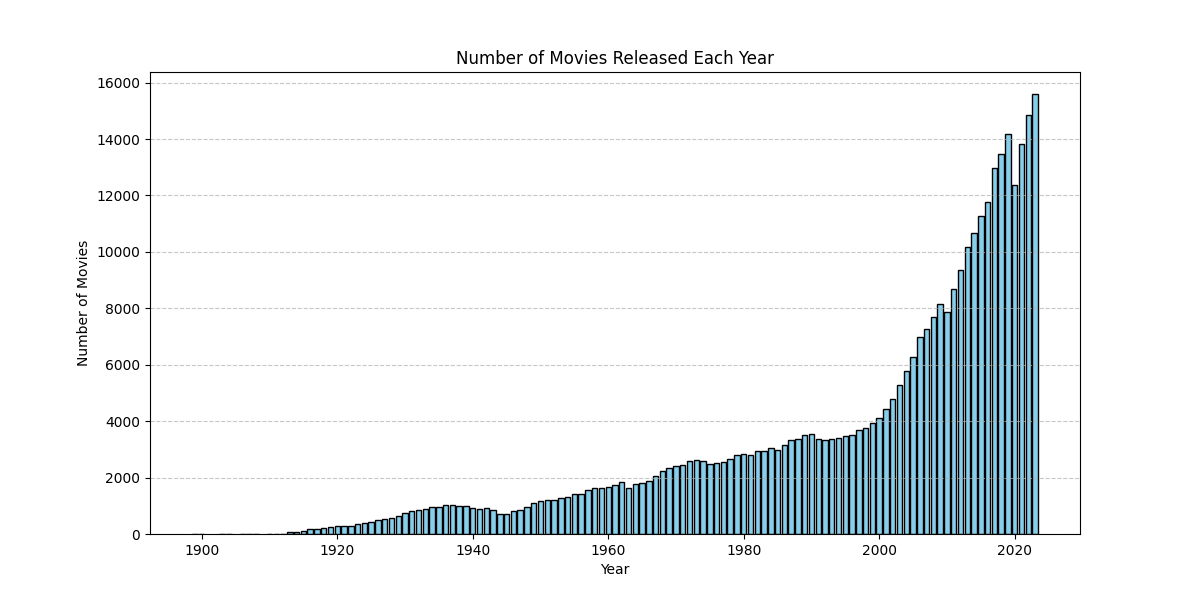
\includegraphics[width=\textwidth]{latex/letterboxd/visualization/movies_count_trend.png}
  \caption{Movies count trend.}
  \label{fig:movies_count_trend}
\end{figure}


\subsection{Most consistent directors (all movies with high ratings)}
This query returns the list of directors found to be more consistent w.r.t the rating of their movies. To do it we used a scoring function (inspired to the tf-idf one) that multiplies the average rating of all movies by the logarithm (applied twice in this case) of their amount.

\inputminted[frame=single,framesep=10pt,breaklines]{cypher}{letterboxd/queries/query2.cypher}

The query returns the following (truncated) result:

\begin{longtable}[!h]{|c|l|c|c|}
\caption{Most consistent directors} \\
\hline
\# & Director & Avg. Rating & Number of Movies \\
\hline
\endfirsthead
\hline
\# & Director & Avg. Rating & Number of Movies \\
\hline
\endhead
\hline
\endfoot
\hline
\endlastfoot

1 & Chuck Jones        & 3.47 & 223 \\
2 & Friz Freleng       & 3.37 & 184 \\
3 & William Hanna      & 3.50 & 124 \\
4 & Joseph Barbera     & 3.50 & 123 \\
5 & Jean-Luc Godard    & 3.54 & 105 \\
6 & Tex Avery          & 3.43 & 108 \\
7 & Dave Fleischer     & 3.43 & 104 \\
8 & Georges Méliès     & 3.20 & 173 \\
9 & Stan Brakhage      & 3.50 & 88  \\
10 & Agnès Varda       & 3.75 & 54  \\
11 & Martin Scorsese   & 3.74 & 54  \\
12 & Ingmar Bergman    & 3.67 & 60  \\
13 & Werner Herzog     & 3.57 & 66  \\
14 & John Ford         & 3.50 & 71  \\
15 & Krzysztof Kieślowski & 3.74 & 44  \\
\end{longtable}

\subsection{Average rating by genre}

We wrote this query because we where interested in finding which genres had better reviewed movies by users on Letterboxd. Having an higher score doesn't necessarily mean that the movies of that category are better, it could alse be that the users of the platform like the genre more.
As we expected, the horror genre is the one populated by low quality movies.

\inputminted[frame=single,framesep=10pt,breaklines]{cypher}{letterboxd/queries/query3.cypher}

The query returns the following result:

\begin{longtable}[!h]{|c|l|c|}
\caption{Genre average ratings} \\
\hline
\# & Genre & Rating \\
\hline
\endfirsthead
\hline
\# & Genre & Rating \\
\hline
\endhead
\hline
\endfoot
\hline
\endlastfoot
1 & Documentary       & 3.52 \\
2 & Music             & 3.44 \\
3 & History           & 3.40 \\
4 & War               & 3.38 \\
5 & Animation         & 3.36 \\
6 & Drama             & 3.33 \\
7 & Western           & 3.29 \\
8 & Crime             & 3.24 \\
9 & Romance           & 3.19 \\
10 & Comedy            & 3.18 \\
11 & Mystery           & 3.18 \\
12 & Fantasy           & 3.15 \\
13 & TV Movie          & 3.11 \\
14 & Family            & 3.11 \\
15 & Adventure         & 3.10 \\
16 & Action            & 3.05 \\
17 & Thriller          & 3.05 \\
18 & Science Fiction   & 3.03 \\
19 & Horror            & 2.92 \\
\end{longtable}

\begin{figure}[!h]
  \centering
  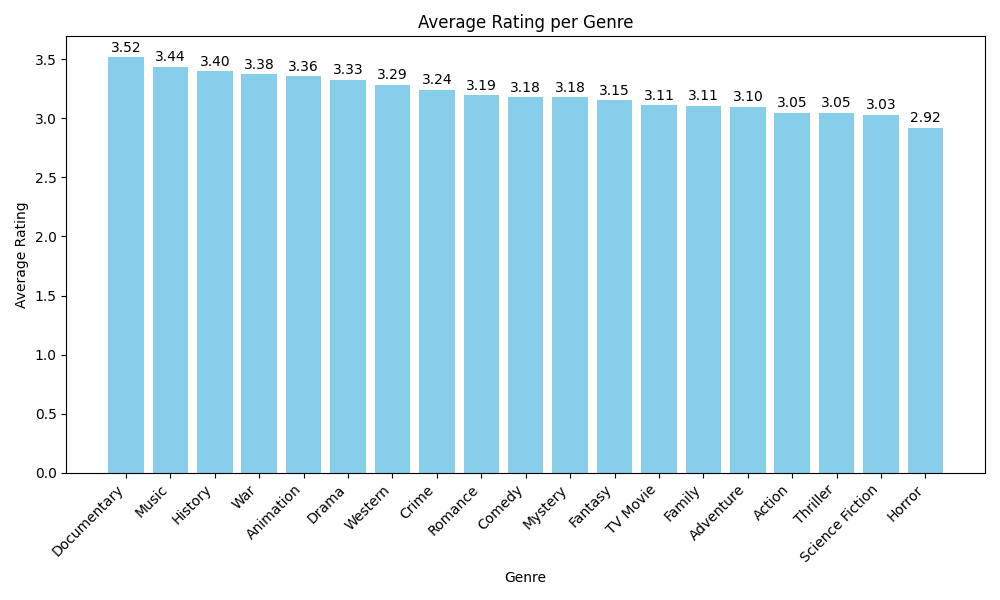
\includegraphics[width=\textwidth]{latex/letterboxd/visualization/average_rating_genre.png}
  \caption{Average rating for genre.}
  \label{fig:average_rating_genre}
\end{figure}

\subsection{Most Productive Studios by Year}

With this query we found the most productive movie studios by year between 1900 and 2023, considering only movies with a rating of 3 or higher (i.e. at least 6/10). The query calculates the number of qualifying movies produced by each studio for each year, returning the year, studio name, and count of movies.
We decided to stop at 5 studios for each year.

\inputminted[frame=single,framesep=10pt,breaklines]{cypher}{letterboxd/queries/query4.cypher}

The query returns the following (truncated to include only 2022 and 2034) result:

\begin{longtable}[!h]{|c|l|c|}
\caption{Top Studios through years by movie count} \\
\hline
Year & Studio & Movies Count \\
\hline
\endfirsthead
\hline
Year & Studio & Movies Count \\
\hline
\endhead
\hline
\endfoot
\hline
\endlastfoot

2023 & France 2 Cinéma & 32 \\
2023 & HBO Documentary Films & 31 \\
2023 & Amazon Studios & 29 \\
2023 & RAI Cinema & 28 \\
2023 & France 3 Cinéma & 27 \\
2022 & ARTE & 38 \\
2022 & France 2 Cinéma & 30 \\
2022 & Amazon Studios & 24 \\
2022 & RAI Cinema & 21 \\
2022 & ARTE France Cinéma & 20 \\

\end{longtable}

\subsection{Genre popularity through the years}

While this query might look simple, it highlights how genres alternated through the years in popularity. It shows how in recent years, while drama has always been a relevant genre, comedy and documentaries have rose in popularity.

\inputminted[frame=single,framesep=10pt,breaklines]{cypher}{letterboxd/queries/query5.cypher}

The output of this query has been truncated to show genre popularity only of 2022 and 2023:

\begin{longtable}[!h]{|c|l|c|}
\caption{Genre popularity through the years} \\
\hline
\textbf{Year} & \textbf{Genre} & \textbf{Count} \\
\hline
\endfirsthead
\hline
\textbf{Year} & \textbf{Genre} & \textbf{Count} \\
\hline
\endhead
\hline
\endfoot
\hline
2023 & Drama & 1423 \\
2023 & Comedy & 751 \\
2023 & Documentary & 557 \\
2023 & Thriller & 263 \\
2023 & Crime & 256 \\
2023 & Animation & 236 \\
2023 & Romance & 233 \\
2023 & Action & 174 \\
2023 & Mystery & 155 \\
2023 & Horror & 153 \\
2023 & Music & 128 \\
2023 & Family & 121 \\
2023 & Science Fiction & 106 \\
2023 & Fantasy & 103 \\
2023 & History & 102 \\
2023 & Adventure & 97 \\
2023 & TV Movie & 64 \\
2023 & War & 40 \\
2023 & Western & 10 \\
2022 & Drama & 1445 \\
2022 & Comedy & 792 \\
2022 & Documentary & 642 \\
2022 & Thriller & 280 \\
2022 & Animation & 266 \\
2022 & Romance & 263 \\
2022 & Crime & 241 \\
2022 & Horror & 199 \\
2022 & Mystery & 183 \\
2022 & Music & 164 \\
2022 & Action & 149 \\
2022 & Fantasy & 135 \\
2022 & Science Fiction & 120 \\
2022 & History & 119 \\
2022 & Family & 105 \\
2022 & Adventure & 92 \\
2022 & TV Movie & 78 \\
2022 & War & 39 \\
2022 & Western & 7 \\
\end{longtable}


\begin{figure}[H]
  \centering
  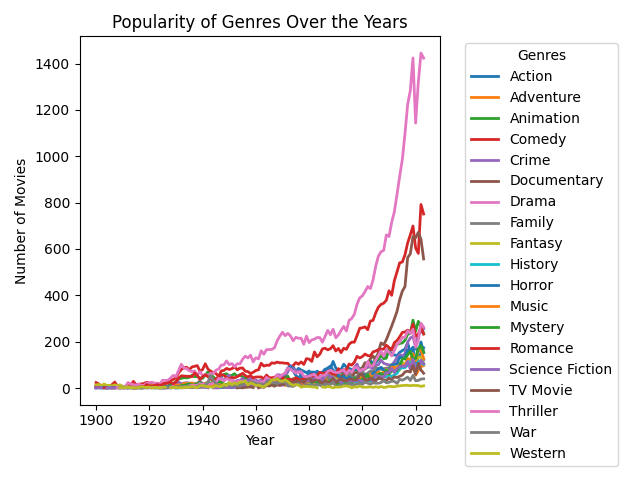
\includegraphics[width=\textwidth]{latex/letterboxd/visualization/genre_popularity.png}
  \caption{Genre popularity through the years.}
  \label{fig:genre_popularity}
\end{figure}

\subsection{Actors who acted in highly rated movies}

Here, we wanted to see which actors (who acted in at least 20 movies) took part in movies that are highly rated. To speed up the query, we considered movies released since 2000 and filmed in USA.

\inputminted[frame=single,framesep=10pt,breaklines]{cypher}{letterboxd/queries/query6.cypher}

You can see the top 10 in the table below.

\begin{table}[h!]
\centering
\begin{tabular}{|l|c|c|}
\hline
\textbf{Actor} & \textbf{Rating} & \textbf{Count} \\ \hline
Viggo Mortensen & 3.64 & 21 \\ \hline
Leonardo DiCaprio & 3.64 & 24 \\ \hline
Gregg Turkington & 3.55 & 23 \\ \hline
Dave Chappelle & 3.53 & 23 \\ \hline
Philip Seymour Hoffman & 3.49 & 33 \\ \hline
Tilda Swinton & 3.49 & 42 \\ \hline
Frank Wood & 3.48 & 23 \\ \hline
Ryan Gosling & 3.47 & 30 \\ \hline
Joaquin Phoenix & 3.46 & 30 \\ \hline
Carey Mulligan & 3.46 & 20 \\ \hline
\end{tabular}
\caption{Actors and their ratings with count of ratings}
\label{tab:actor_ratings}
\end{table}


\newpage
\subsection{Number of good movies by years and by  countries they were filmed in}

Here, we decided to find how many good movies were filmed across countries and years. To filter good movies, we decided to include only movies with a rating of at least 3.8/5.0.
\inputminted[frame=single,framesep=10pt,breaklines]{cypher}{letterboxd/queries/query7.cypher}

\begin{table}[H]
\centering
\caption{Count of good movies by country (truncated to include only some countries in 2023)}
\begin{tabular}{|l|c|c|}
\hline
\textbf{Year} & \textbf{Country}     & \textbf{Movie Count} \\
\hline
2023          & USA                 & 97                   \\
2023          & UK                  & 38                   \\
2023          & France              & 28                   \\
2023          & South Korea         & 27                   \\
2023          & Japan               & 24                   \\
2023          & Germany             & 11                   \\
2023          & India               & 8                    \\
2023          & Spain               & 8                    \\
2023          & Brazil              & 7                    \\
2023          & Italy               & 7                    \\
2023          & Argentina           & 6                    \\
2023          & Australia           & 4                    \\
2023          & Belgium             & 4                    \\
2023          & China               & 3                    \\
2023          & Ireland             & 3                    \\
2023          & Sweden              & 3                    \\
2023          & Canada              & 3                    \\
2023          & Poland              & 3                    \\
2023          & Egypt               & 2                    \\
2023          & Norway              & 2                    \\ \hline
\end{tabular}
\end{table}

Over the years, the number of movies with high ratings made by each country has gone up. But, when we look at the first query, it shows that the average ratings have gone down. This shows that even though more good movies are being made, the average review rating is dropping.


\begin{figure}[H]
  \centering
  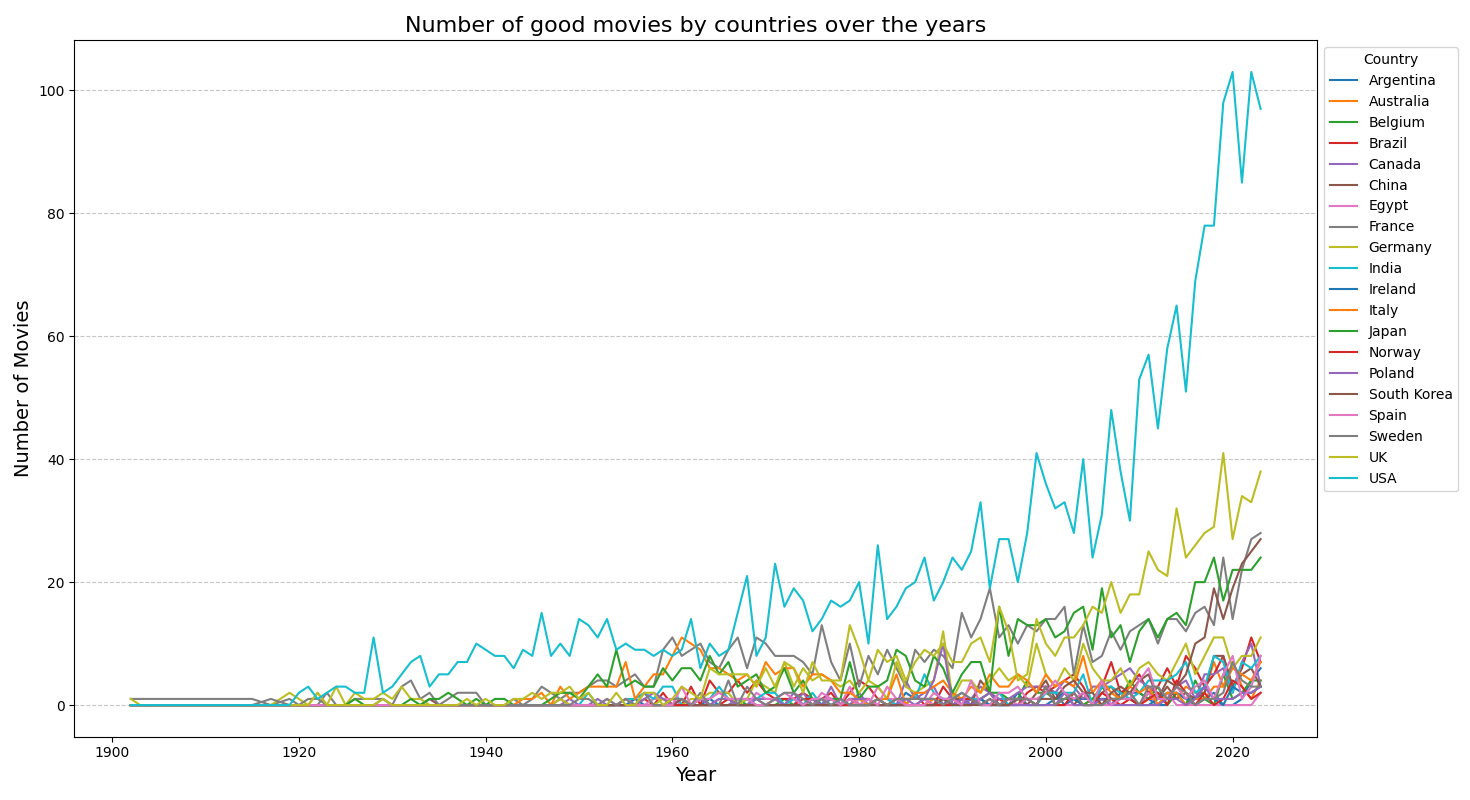
\includegraphics[width=\textwidth]{latex/letterboxd/visualization/good_movies_by_country.png}
  \caption{Count of good movies by country they were filmed in.}
  \label{fig:good_movies_by_countries}
\end{figure}

\subsection{Frequent actor-genre pairings (since 2000)}

Most actors often star in movies of the same genre, so we wanted to find the ones that are particularly "loyal" to a certain genre. To do it we used the following query:

\inputminted[frame=single,framesep=10pt,breaklines]{cypher}{letterboxd/queries/query8.cypher}

The truncated output with the first 20 pairings can be found in table \ref{tab:actor_genres}.

\begin{table}[h!]
\centering
\begin{tabular}{|l|l|c|}
\hline
\textbf{Actor} & \textbf{Genre} & \textbf{Appearances} \\ \hline
Tim Heidecker & Comedy & 19 \\ \hline
Tom Kenny & Comedy & 18 \\ \hline
Tilda Swinton & Drama & 17 \\ \hline
Jason Schwartzman & Comedy & 16 \\ \hline
Michael Shannon & Drama & 16 \\ \hline
Matt Damon & Drama & 15 \\ \hline
Bill Camp & Drama & 15 \\ \hline
Stan Lee & Action & 15 \\ \hline
Kathleen Barr & Family & 15 \\ \hline
Bill Murray & Comedy & 15 \\ \hline
Michael Stuhlbarg & Drama & 15 \\ \hline
Louis C.K. & Comedy & 15 \\ \hline
Cate Blanchett & Drama & 15 \\ \hline
Stan Lee & Adventure & 14 \\ \hline
Dee Bradley Baker & Comedy & 14 \\ \hline
Gregg Turkington & Comedy & 14 \\ \hline
Lauren Lopez & Comedy & 14 \\ \hline
Willem Dafoe & Drama & 14 \\ \hline
David Cross & Comedy & 14 \\ \hline
Jack Black & Comedy & 13 \\ \hline
\end{tabular}
\caption{Actors, their genres, and number of appearances}
\label{tab:actor_genres}
\end{table}

\subsection{Frequent actor-director pairings in movies with good ratings and produced in USA
}

The original idea behind this query was to find all pairings actor-director, but since the dataset was too big to do so (even with the help of indexes to speed up the query), we decided to restrict to movies filmed in USA and with a rating of at least 4/5.

\inputminted[frame=single,framesep=10pt,breaklines]{cypher}{letterboxd/queries/query9.cypher}

The result produced by the query is not surprising, as there are pairings like De Niro-Scorsese and DiCaprio-Tarantino.

\begin{table}[h!]
\centering
\begin{tabular}{|l|l|c|}
\hline
\textbf{Actor} & \textbf{Director} & \textbf{Count} \\ \hline
Alfred Hitchcock & Alfred Hitchcock & 9 \\ \hline
Tim Heidecker & Eric Notarnicola & 7 \\ \hline
Gregg Turkington & Eric Notarnicola & 7 \\ \hline
Joe Estevez & Eric Notarnicola & 6 \\ \hline
Martin Scorsese & Martin Scorsese & 6 \\ \hline
Robert De Niro & Martin Scorsese & 6 \\ \hline
Charlie Chaplin & Charlie Chaplin & 6 \\ \hline
Henry Bergman & Charlie Chaplin & 5 \\ \hline
Samuel L. Jackson & Quentin Tarantino & 5 \\ \hline
Mark Proksch & Eric Notarnicola & 5 \\ \hline
Robert Duvall & Francis Ford Coppola & 5 \\ \hline
Bess Flowers & Alfred Hitchcock & 5 \\ \hline
Buster Keaton & Buster Keaton & 5 \\ \hline
Michael Caine & Christopher Nolan & 4 \\ \hline
Russ Fega & Christopher Nolan & 4 \\ \hline
Uma Thurman & Quentin Tarantino & 4 \\ \hline
Quentin Tarantino & Quentin Tarantino & 4 \\ \hline
Leonardo DiCaprio & Martin Scorsese & 4 \\ \hline
Kyle MacLachlan & David Lynch & 4 \\ \hline
Jack Nance & David Lynch & 4 \\ \hline
\end{tabular}
\caption{Actor-Director pairings}
\label{tab:actor_director_pairings}
\end{table}

 \subsection{Theatrical vs Digital releases}

 For the last query, we wanted to see how movie releases changed since the introduction of online renting and streaming.

 \inputminted[frame=single,framesep=10pt,breaklines]{cypher}{letterboxd/queries/query10.cypher}

 \begin{table}[!h]
\centering
\begin{tabular}{|r|l|r|}
\hline
\textbf{Release Year} & \textbf{Release Type} & \textbf{Total Movies} \\
\hline
2023 & Theatrical & 12161 \\
2023 & Digital & 11671 \\
2022 & Digital & 11033 \\
2022 & Theatrical & 10984 \\
2021 & Digital & 12381 \\
2021 & Theatrical & 10072 \\
2020 & Digital & 12645 \\
2020 & Theatrical & 9466 \\
2019 & Theatrical & 12323 \\
2019 & Digital & 7174 \\
2018 & Theatrical & 12629 \\
2018 & Digital & 5766 \\
\hline
\end{tabular}
\caption{Release Year, Release Type, and Total Movies}
\end{table}

 By looking at the graph we generated from the query, we can notice how during covid digital releases overtook theatrical ones (as expected) and, more in general, how digital releases have been on the rise since early 2000s.

\begin{figure}[!h]
  \centering
  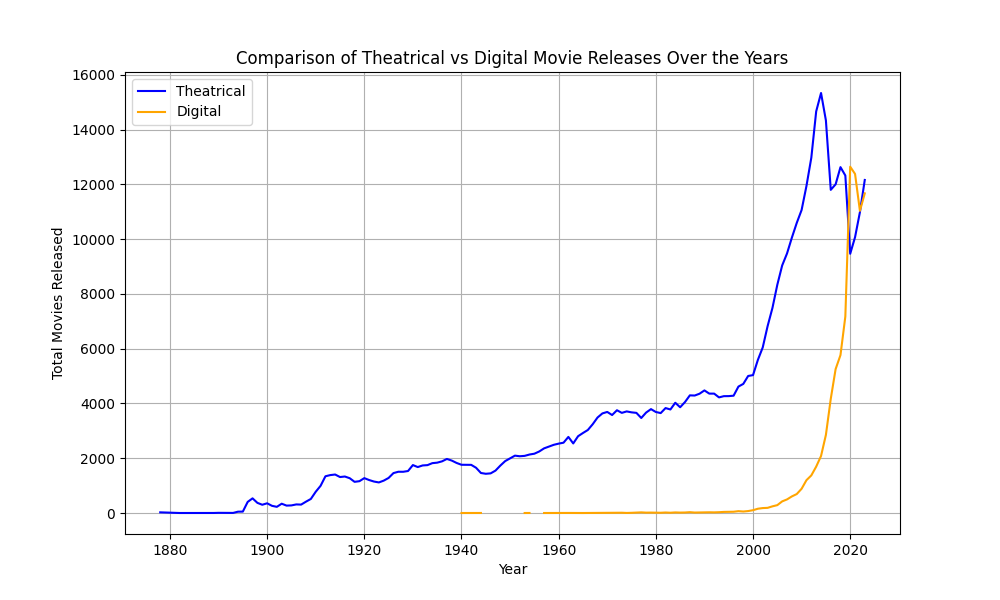
\includegraphics[width=\textwidth]{latex/letterboxd/visualization/releases.png}
  \caption{Digital vs Theatrical releases.}
  \label{fig:releases}
\end{figure}


\section{Formula 1 dataset queries}
\subsection{List of drivers sorted based on wins count}
Drivers in Formula 1 dream since being children about winning their first race in the most important category of the motorsport world.
Through this query we aim to seek who the most winning drivers ever are, and we list the top 10. 

\vspace{0.5cm}
\inputminted[frame=single,framesep=10pt,breaklines]{python}{formula1/queries/query1.py}

\newpage
\begin{table}[!h]
    \centering
    \begin{tabular}{|l|l|r|}
        \hline
        \textbf{Name} & \textbf{Surname} & \textbf{Wins} \\
        \hline
        Lewis & Hamilton & 104 \\
        Michael & Schumacher & 91 \\
        Max & Verstappen & 61 \\
        Sebastian & Vettel & 53 \\
        Alain & Prost & 51 \\
        Ayrton & Senna & 41 \\
        Fernando & Alonso & 32 \\
        Nigel & Mansell & 31 \\
        Jackie & Stewart & 27 \\
        Niki & Lauda & 25 \\
        \hline
    \end{tabular}
    \caption{Top 10 drivers in terms of race wins}
\end{table}


\subsection{Most important nations in Formula 1}
For the next query, divided into two, our objective is to identify the most relevant countries in Formula 1. The sport is always perceived as being Europe-centric, and we will try to confirm or disprove the theory.

\vspace{0.5cm}
\inputminted[frame=single,framesep=10pt,breaklines]{python}{formula1/queries/query2.py}

\newpage
\begin{table}[!h]
    \centering
    \begin{tabular}{|r|c|}
        \hline
        \textbf{Country} & \textbf{Drivers Count} \\
        \hline
        British & 166 \\
        American & 158 \\
        Italian & 99 \\
        French & 73 \\
        German & 50 \\
        Brazilian & 32 \\
        Swiss & 23 \\
        Argentine & 23 \\
        Belgian & 23 \\
        South African & 23 \\
        \hline
    \end{tabular}
    \caption{Count of drivers by country}
\end{table}

\begin{table}[!h]
    \centering
    \begin{tabular}{|r|c|}
        \hline
        \textbf{Country} & \textbf{Constructors Count} \\
        \hline
        British & 86 \\
        American & 38 \\
        Italian & 30 \\
        French & 13 \\
        German & 10 \\
        Brazilian & 5 \\
        Swiss & 5 \\
        Argentine & 3 \\
        Belgian & 3 \\
        South African & 2 \\
        \hline
    \end{tabular}
    \caption{Count of constructors by country}
\end{table}

The results show a big percentage of European countries, thus confirming what is perceived of the sport.


\subsection{Most difficult tracks for overtaking}
Different circuits have different characteristics, including track width. This implies overtaking another driver also depends on track features. Let us try to infer on which circuits it is more difficult to fight another driver, counting the races that were won by starting from pole position.

\vspace{0.5cm}
\inputminted[frame=single,framesep=10pt,breaklines]{python}{formula1/queries/query3.py}

\newpage
\begin{table}[!h]
    \centering
    \begin{tabular}{|c|c|c|c|}
        \hline
        \textbf{Circuit} & \textbf{Wins from Pole} & \textbf{Races Count} & \textbf{Wins Percentage} \\
        \hline
        Montmelò & 24 & 34 & 0.71 \\
        Istanbul & 6 & 9 & 0.67 \\
        Abu Dhabi & 10 & 15 & 0.67 \\
        Marina Bay & 9 & 14 & 0.64 \\
        Le Castellet & 11 & 18 & 0.61 \\
        Valencia & 3 & 5 & 0.6 \\
        Shanghai & 10 & 17 & 0.59 \\
        Suzuka & 18 & 34 & 0.53 \\
        New York State & 10 & 20 & 0.5 \\
        Liverpool & 3 & 6 & 0.5 \\
        \hline
    \end{tabular}
    \caption{Ratio of races won from pole position}
\end{table}

Tracks related to a high percentage should be the ones having less overtaking possibilities. As seen from the results, that is true for the majority of them, but not for all: the track found in Istanbul presents a lot of overtaking spots. Additionally, some tracks that offer very few overtaking spots in reality, such as Monaco, are unexpectedly missing from the list.

\subsection{Wins from different starting positions}
We now know the list of circuits on which it is most difficult to overtake, discovered by exploring how many races were won from pole position. One might ask about the other starting positions and how many races where won from them. That is what we will try to understand with the next query.

\vspace{0.5cm}
\inputminted[frame=single,framesep=10pt,breaklines]{python}{formula1/queries/query4.py}

\vspace{0.5cm}
\begin{table}[!h]
    \centering
    \begin{tabular}{|c|c|}
        \hline
        \textbf{Grid} & \textbf{Wins Count} \\
        \hline
        1 & 476 \\
        2 & 265 \\
        3 & 136 \\
        4 & 66 \\
        5 & 49 \\
        6 & 40 \\
        7 & 23 \\
        8 & 17 \\
        9 & 5 \\
        10 & 12 \\
        11 & 5 \\
        12 & 3 \\
        13 & 4 \\
        14 & 7 \\
        15 & 1 \\
        16 & 2 \\
        17 & 2 \\
        18 & 1 \\
        19 & 1 \\
        22 & 1 \\
        \hline
    \end{tabular}
    \caption{Count of wins based on the starting position}
\end{table}

As expected, the likelihood of winning decreases progressively with the starting positions further from pole.

\newpage
\subsection{Evolution of Formula 1 lap times}
Being the pinnacle of motorsport, Formula 1 is in continuous evolution: lap times are the first element in the Formula 1 world which is affected. It might be very interesting to know the entity of this change throughout the years.

To do so, results from qualifying on one of the most famous and long lasting tracks, Silverstone, are used.

\vspace{0.5cm}
\inputminted[frame=single,framesep=10pt,breaklines]{python}{formula1/queries/query5.py}

\begin{figure}[!h]
  \centering
  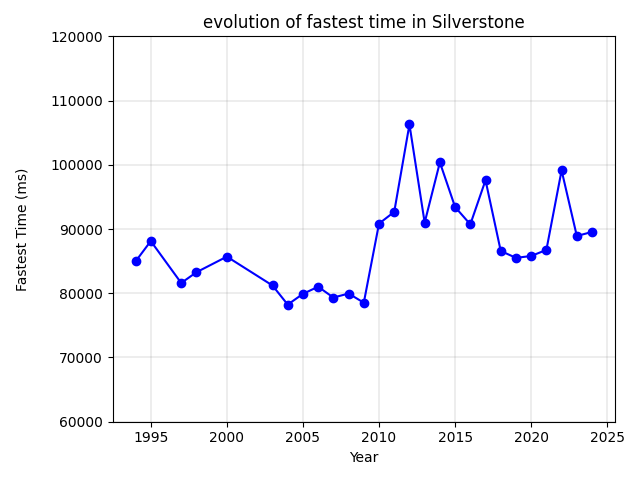
\includegraphics[width=0.75\textwidth]{latex/formula1/visualization/query5.png}
  \caption{Evolution of lap times in Silverstone}
  \label{fig:releases}
\end{figure}

Unfortunately, qualifying data is only available from year 1994 onwards. The curve generally shows a descending trend, with the exception around 2014, when new car regulations were introduced. Random peaks in the diagram are related to years where qualifying sessions were carried out in wet conditions, that is, while it was raining.


\subsection{Evolution of Formula 1 pit stops times}
Formula 1 is about finding perfection in every aspect of racing, including pit stops. The graph shows the evolution of pit stop times in the Monza circuit. Unfortunately, pit stop data is only available from 2011 onwards, for all circuits.

\vspace{0.5cm}
\inputminted[frame=single,framesep=10pt,breaklines]{python}{formula1/queries/query6.py}

\begin{figure}[!h]
  \centering
  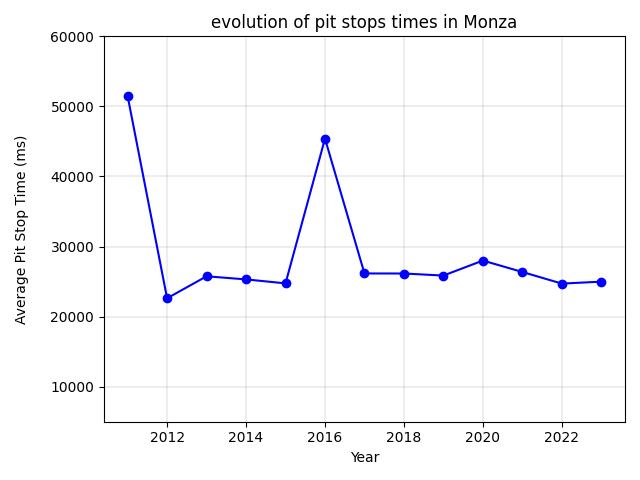
\includegraphics[width=0.75\textwidth]{latex/formula1/visualization/query6.png}
  \caption{Evolution of pit stop times in Monza}
  \label{fig:releases}
\end{figure}

Over the past decade, pit stop times in Formula 1 have remained unchanged. This stagnation can be attributed to two main factors. First, teams have reached the physical lower limit of what is achievable. Second, the FIA, the governing body that establishes Formula 1 regulations, periodically introduces new rules for pit stops, preventing teams from fully optimizing their processes.


\subsection{Drivers analysis}
In \textit{Section 4.2.1}, a query was performed to identify the drivers with most wins during their career. However, in the world of motorsport, victories often depend on having a competitive car, making it impossible to determine the best drivers solely from this list.

To uncover the top talents ever, a more reliable metric can be obtained by comparing drivers to their teammates, who drive identical cars: the higher the percentage of races in which a driver beats their teammate, the greater their talent is likely to be.

For the analysis, only drivers completing at least 100 races (around 5-6 years of career) were considered.

\vspace{0.5cm}
\inputminted[frame=single,framesep=10pt,breaklines]{python}{formula1/queries/query7.py}

\vspace{0.5cm}
\begin{table}[!h]
    \centering
    \begin{tabular}{|c|c|c|c|c|}
        \hline
        \textbf{Name} & \textbf{Surname} & \textbf{Wins} & \textbf{Duels} & \textbf{Win Percentage} \\
        \hline
        Duane & Carter & 93 & 117 & 0.79 \\
        Juan & Fangio & 189 & 246 & 0.77 \\
        Bill & Vukovich & 80 & 107 & 0.75 \\
        Jim & Clark & 161 & 218 & 0.74 \\
        Art & Cross & 78 & 107 & 0.73 \\
        Max & Verstappen & 142 & 197 & 0.72 \\
        Mika & Salo & 78 & 111 & 0.70 \\
        Bruce & McLaren & 174 & 251 & 0.69 \\
        Jack & McGrath & 94 & 137 & 0.69 \\
        Fernando & Alonso & 265 & 392 & 0.68 \\
        \hline
    \end{tabular}
    \caption{Percentage of duels with teammate won}
\end{table}


\subsection{Shift of teams' dominance}
Now, our focus is on teams rather than drivers. How did the most important constructors, i.e. the ones that won the most championships, behave over the course of the years?

It is possible to study it by analyzing their final positions in the constructors championships through time.

\vspace{0.5cm}
\inputminted[frame=single,framesep=10pt,breaklines]{python}{formula1/queries/query8.py}

\newpage
\begin{figure}[!h]
  \centering
  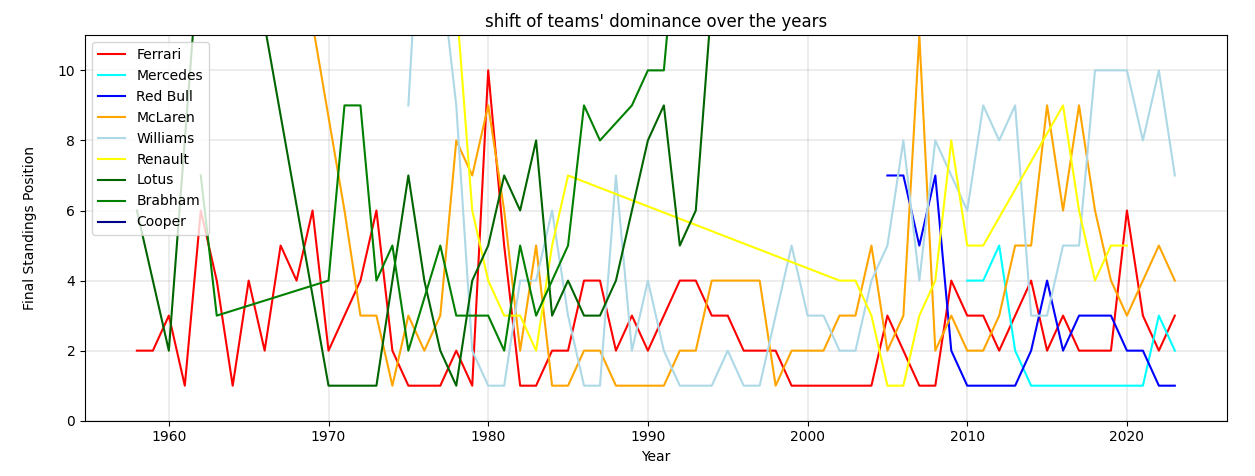
\includegraphics[width=\textwidth]{latex/formula1/visualization/query8.png}
  \caption{Shift of teams' dominance over the years}
  \label{fig:releases}
\end{figure}

Both Mercedes and Red Bull teams managed to finish the year in a good position since they entered the world of Formula 1.

Williams and McLaren teams, instead, fluctuated more in terms of performances, but also started their career a very long time ago, making them experienced and reliable.

However, there is one team, Ferrari, who managed to keep a good position during their stint even though they never missed a race since 1950, making them the most influential team to ever exist in Formula 1.


\subsection{Importance of car in Formula 1}
In Formula 1, it is only possible to win if given a car capable of winning. With the following query we count the number of world champion drivers who won with a car that also won the world constructors championship, trying to infer how important a car is for a Grand Prix win.

Note: due to the limitations regarding the sorting functionality for the MongoDB Atlas free-tier, we were obliged to restrict the number of entries. In particular, we only considered championships from 1975 onwards.

\vspace{0.5cm}
\inputminted[frame=single,framesep=10pt,breaklines]{python}{formula1/queries/query9.py}

\vspace{0.5cm}
\begin{table}[!h]
    \centering
    \begin{tabular}{|c|c|}
        \hline
        \textbf{Both Championships Winners}
        & 38 \\
        \hline
    \end{tabular}
    \caption{Times both championships were won by the same team}
\end{table}

Only seasons since 1975 were considered: this implies that $78\%$ of driver championships were won with the fastest car on the grid.

We also wanted to showcase the code for displaying the last ten occasions in which both championships were won by a team. If we were to run the commented code instead of the "\$count" function, the table below would be generated.

\vspace{0.5cm}
\begin{table}[!h]
    \centering
    \begin{tabular}{|c|c|c|c|c|}
        \hline
        \textbf{Year} & \textbf{Name} & \textbf{Surname} & \textbf{Constructor} \\
        \hline
        2023 & Max & Verstappen & Red Bull \\
        2022 & Max & Verstappen & Red Bull \\
        2020 & Lewis & Hamilton & Mercedes \\
        2019 & Lewis & Hamilton & Mercedes \\
        2018 & Lewis & Hamilton & Mercedes \\
        2017 & Lewis & Hamilton & Mercedes \\
        2016 & Nico & Rosberg & Mercedes \\
        2015 & Lewis & Hamilton & Mercedes \\
        2014 & Lewis & Hamilton & Mercedes \\
        2013 & Sebastian & Vettel & Red Bull \\
        \hline
    \end{tabular}
    \caption{Times both championships were won by the same team}
\end{table}

In the last 12 years, a championship was won with a non championship-winning car only one time.


\subsection{Most Grand Prix starts for Ferrari}
As seen from \textit{Section 4.2.8}, Ferrari is the greatest constructor in Formula 1, ever.

To conclude our dataset analysis, we can identify the top 15 drivers in terms of races completed for the most influential team in Formula 1, and how many of these were eventually won.

\vspace{0.5cm}
\inputminted[frame=single,framesep=10pt,breaklines]{python}{formula1/queries/query10.py}

\vspace{0.5cm}
\begin{table}[!h]
    \centering
    \begin{tabular}{|c|c|c|c|}
        \hline
        \textbf{Name} & \textbf{Surname} & \textbf{Wins} & \textbf{Races} \\
        \hline
        Michael & Schumacher & 72 & 181 \\
        Kimi & Raikkonen & 10 & 152 \\
        Felipe & Massa & 11 & 140 \\
        Sebastian & Vettel & 14 & 119 \\
        Charles & Leclerc & 6 & 116 \\
        Rubens & Barrichello & 9 & 104 \\
        Fernando & Alonso & 11 & 96 \\
        Gerharg & Berger & 5 & 96 \\
        Michele & Alboreto & 3 & 80 \\
        Jean & Alesi & 1 & 79 \\
        Carlos & Sainz & 3 & 77 \\
        Clay & Regazzoni & 4 & 73 \\
        Gilles & Villeneuve & 6 & 67 \\
        Eddie & Irvine & 4 & 65 \\
        Niki & Lauda & 15 & 58 \\
        \hline
    \end{tabular}
    \caption{Most important drivers for Ferrari}
\end{table}

%-------------------------------------------------------------------------
%	APPENDICES
%-------------------------------------------------------------------------

\cleardoublepage

% % LIST OF FIGURES
\listoffigures

% % LIST OF TABLES
\listoftables

\cleardoublepage

\end{document}
